\documentclass[11pt]{article}
% Libraries.
\usepackage{amsmath}
\usepackage{amssymb}
\usepackage{pgfplots}
\usepackage{graphicx}
\usepackage{enumitem}
\usepackage{hyperref}
\usepackage{fancyhdr}
\usepackage{perpage}
\usepackage{float}
\usepackage{esint}
\usepackage[margin=1.5cm]{geometry}

% Property settings.
\MakePerPage{footnote}
\pagestyle{headings}

% Commands
\newcommand{\ti}[1]{\textit{#1}}
\newcommand{\tb}[1]{\textbf{#1}}
\newcommand{\mb}[1]{\mathbb{#1}}
\newcommand{\mc}[1]{\mathcal{#1}}
\newcommand{\bx}[0]{\mathbf{x}}
\newcommand{\bv}[0]{\mathbf{v}}
\newcommand{\bw}[0]{\mathbf{w}}
\newcommand{\real}[0]{\mathbb{R}}
\newcommand{\under}[1]{\underline{#1}}
\newcommand{\proof}[0]{\textit{\underline{proof:} }}
\newcommand{\func}[3]{\tb{#1}: {#2} \rightarrow {#3} }
\newcommand{\vx}[0]{\tb{x}}
\newcommand{\vy}[0]{\tb{y}}
\newcommand{\vz}[0]{\tb{z}}
\newcommand{\vo}[0]{\tb{0}}
\newcommand{\va}[0]{\tb{a}}
\newcommand{\vb}[0]{\tb{b}}
\newcommand{\vc}[0]{\tb{c}}
\newcommand{\ve}[0]{\tb{e}}
\newcommand{\vm}[0]{\tb{m}}
\newcommand{\vh}[0]{\tb{h}}
\newcommand{\vf}[0]{\tb{F}}
\newcommand{\vi}[0]{\tb{i}}
\newcommand{\vj}[0]{\tb{j}}
\newcommand{\vk}[0]{\tb{k}}
\newcommand{\vr}[0]{\tb{r}}
\newcommand{\vg}[0]{\tb{G}}
\newcommand{\vn}[0]{\tb{n}}
\newcommand{\vu}[0]{\tb{u}}
\newcommand{\vv}[0]{\tb{v}}
\newcommand{\vL}[0]{\tb{L}}
\newcommand{\ff}[0]{\tb{f}}
\newcommand{\fg}[0]{\tb{g}}
\newcommand{\p}[0]{\partial}
\newcommand{\qed}[0]{$\hfill\blacksquare$}
\newcommand{\qerat}{\tag*{$\blacksquare$}}
\newcommand{\lima}{\underset{\vx \rightarrow \va}{\lim}}
\usepackage{amsmath}% http://ctan.org/pkg/amsmath
\newcommand{\notimplies}{%
  \mathrel{{\ooalign{\hidewidth$\not\phantom{=}$\hidewidth\cr$\implies$}}}}
\newcommand{\q}[0]{\textcolor{red}{???}}
\newcommand{\tspace}[0]{T_{x_0}}
\newcommand{\tanspace}[0]{T_{x_0}M}
% Attr.
\title{CSC311 \\ Lecture Notes}
\author{Yuchen Wang}
\date{\today}

\begin{document}
    \maketitle
    \tableofcontents
    \newpage
    
    
\section{Lecture 9 - k-Means and EM Algorithm}
\subsection{Latent variable models}
\tb{Assumption}: data depends on some latent variables that are never observed. \\
\tb{Example}: PCA (Even though data is very high dimensional, it can be well represented in low dimensions.)

\subsection{Clustering}
Grouping data points into clusters, with no observed labels, is called \under{clustering}. \\
Samples within a cluster are similar to each other, and samples in different clusters are dissimilar. It is an unsupervised technique. Such a distribution is multimodal, since it has multiple modes, or regions of high probability mass.
    
\paragraph{Example} Clustering machine learning papers based on topic (deep learning, Bayesian models, etc)

\subsection{Clustering Problem}
\paragraph{Assumptions}
\begin{enumerate}
	\item The data $\{\vx^{(1)}, \hdots, \vx^{(N)}\}$ lives in a Euclidean space, $\vx^{(n)} \in \real^D$
	\item Each data point belongs to one of K clusters
	\item The data points from the same cluster are similar (i.e. close in Euclidean distance)
\end{enumerate}

\subsection{K-means}
\paragraph{Objective}
Find cluster centers $\{\vm_k\}_{k=1}^K$ and assignments $\{\vr^{(n)}\}_{n=1}^N$ to minimize the sum of squared distances of data points $\{\vx^{(n)}\}$ to their assigned cluster centers.
\begin{enumerate}
	\item Data sample $n = 1, \hdots, N: \vx^{(n)} \in \real^D$ (observed)
	\item Cluster center $k = 1, \hdots, K: \vm_k \in \real^D$ (not observed)
	\item Responsibilities: Cluster assignment for sample $n$: $\vr^{(n)} \in \real^K$ 1-of-K encoding (not observed)
\end{enumerate}
\paragraph{Objective Mathematically}
$$\begin{array}{l}{\min _{\left\{\mathbf{m}_{k}\right\},\{\mathbf{r}^{(n)}\}} J\left(\left\{\mathbf{m}_{k}\right\},\{\mathbf{r}^{(n)}\}\right)=\min _{\left\{\mathbf{m}_{k}\right\},\{\mathbf{r}^{(n)}\}} \sum_{n=1}^{N} \sum_{k=1}^{K} r_{k}^{(n)}\left\|\mathbf{m}_{k}-\mathbf{x}^{(n)}\right\|^{2}} \\ {\text { where } r_{k}^{(n)}=\mathbb{I}\left[\mathbf{x}^{(n)} \text { is assigned to cluster } k\right], \text { i.e., } \mathbf{r}^{(n)}=[0, \ldots, 1, \ldots, 0]^{\top}}\end{array}$$

\paragraph{Notes}
Finding an optimal solution is an \textcolor{blue}{NP-hard} problem.
    
\subsubsection{K-means Algorithm}
\tb{Initialization: } Set K cluster means $\vm_1, \hdots, \vm_K$ to random values \\
Repeat until convergence (until assignments do not change): \\
\tb{Assignment: } Optimize $J$ w.r.t. $\{\vr\}:$ Each data point $\vx^{(n)}$ assigned to nearest center
$$\hat{k}^{(n)} = \underset{k}{argmin} ||\vm_k - \vx^{(n)}||^2$$
and \tb{Responsibilities} (1-hot encoding) 
$$r_k^{(n)} = \mb{I}[\hat{k}^{(n)} = k]$$ for $k = 1,\hdots,K$\\
\tb{Refitting: } Optimize J w.r.t. $\{\vm\}$: Each center is set to mean of data assigned to it 
$$\vm_k = \frac{\sum_k r_k^{(n)}\vx^{(n)}}{\sum_n r_k^{(n)}}$$

\paragraph{Performance}
\begin{enumerate}
	\item K-means algorithm reduces the cost at each iteration.
	\item The objective $J$ is non-convex, so coordinate descent on $J$ is not guaranteed to converge to the global minimum (\textcolor{red}{solution: we could try many random starting points})
\end{enumerate}

\subsection{Soft K-means}
One cluster may have a responsibility of $.7$ for a datapoint and another may have a responsibility of $.3$. This allows a cluster to use more information about the data in the refitting step.

\subsubsection{Soft K-means Algorithm}
\tb{Initialization: } Set K cluster means $\vm_1, \hdots, \vm_K$ to random values \\
Repeat until convergence (until assignments do not change):\\
\tb{Assignment: } Each data point $n$ given soft ``degree of assignment" to each cluster mean $k$, based on responsibilities
$$r_k^{(n)} = \frac{\exp[-\beta||\vm_k - \vx^{(n)}||^2]}{\sum_j \exp[-\beta||\vm_j - \vx^{(n)}||^2}]$$
where $\beta$ is a hyperparameter.
$$\implies \vr^{(n)} = softmax(-\beta\{\vm_k - \vx^{(n)}||^2 \} _{k=1}^K)$$
\tb{Refitting: } Model parameters, means, are adjusted to match sample means of datapoints they are responsible for:
$$\vm_k = \frac{\sum_k r_k^{(n)}\vx^{(n)}}{\sum_n r_k^{(n)}}$$

\paragraph{Remarks}
As $\beta \rightarrow \infty$, soft k-Means converges to hard k-Means.

\subsection{A Generative View of Clustering}
Imagine that the data was produced by a generative model, then adjust the model parameters using MLE, i.e., maximize the probability that it would product exactly the data we observed. \\
Assume a datapoint $\vx$ is generated as followw:
\begin{enumerate}
	\item Choose a cluster $z$ from $\{1,\hdots, K\}$ such that $p(z=k) = \pi_k$
	\item Given $z$, sample $\vx$ from a Gaussian distribution $\mc{N}(\vx|\mu_z, I)$
\end{enumerate}
Can also be written:
$$p(z=k) = \pi_k$$
$$p(\vx|z=k) = \mc{N}(\vx|\mu_k, I)$$
This defines joint distribution $p(z, \vx) = p(z)p(\vx|z)$ with parameters $\{\pi_k, \mu_k\}_{k=1}^K$, and the marginal of $\vx$ is given by $p(\vx) = \sum_z p(z,x)$. $p(z = k | \vx)$ can be computed using Bayes rule.

\begin{align} p(z=k | \mathbf{x}) &=\frac{p(z=k) p(\mathbf{x} | z=k)}{p(\mathbf{x})} \\ &=\frac{p(z=k) p(\mathbf{x} | z=k)}{\sum_{j=1}^{K} p(z=j) p(\mathbf{x} | z=j)} \\ &=\frac{\pi_{k} \mathcal{N}\left(\mathbf{x} | \boldsymbol{\mu}_{k}, \mathbf{I}\right)}{\sum_{j=1}^{K} \pi_{j} \mathcal{N}\left(\mathbf{x} | \boldsymbol{\mu}_{j}, \mathbf{I}\right)} \end{align}
This tells us the probability $\vx$ came from the $k$th cluster

\paragraph{Choose $\pi_k$ and $\mu_k$}
Choose parameters to maximize likelihood of observed data. Given data $\mc{D} = \{\vx^{(n)}\}_{n=1}^N$, choose parameters to maximize:
$$\log p(\mc{D}) = \sum_{n=1}^N \log p(\vx^{(n)})$$
Find $p(\vx)$ by marginalizing out $z$:
$$p(\vx) = \sum_{k=1}^Kp(z=k, \vx) = \sum_{k=1}^Kp(z=k)p(\vx|z=k) = \sum_{k=1}^K\pi_k\mc{N}(\vx|\mu_k, I)$$
which is an example of \under{Gaussian Mixture Model (GMM)}, and $pi_k$ are known as the \under{mixing coefficients}.
\paragraph{Note}
If we allow arbitrary covariance matrices, GMMs are \under{universal approximators of densities} (if you have enough Gaussians). Even diagonal GMMs are universal approximators.

\paragraph{Maximum Likelihood objective}
$$\log p (\mc{D}) = \sum_{n=1}^N \log p(\vx^{(n)}) = \sum_{n=1}^N \log \left ( \sum_{k=1}^K \pi_k \mc{N}(\vx^{(n)}|\mu_k,I)\right )$$

\subsection{Expectation-Maximization algorithm}
\begin{enumerate}
	\item \tb{E-step}: Compute the posterior probabilities $r_k^{(n)} = p(z^{(n)} = k | \vx^{(n)})$ given our current model - i.e. How much do we think a cluster is responsible for generating a datapoint.
	\item \tb{M-step}: Use the equations on the last slide to update the parameters, assuming $r_k^{(n)}$ are held fixed- change the parameters of each Gaussian to maximize the probability that it would generate the data it is currently responsible for.
\end{enumerate}
Mathematically,
\begin{enumerate}
	\item \tb{E-step}: Evaluate the responsibilities $r_k^{(n)}$ given current parameters
	$$r_k^{(n)} = p(z^{(n)} = k | \vx^{(n)}) = \frac{\hat{\pi}_k\mc{N}(\vx^{(n)}|\hat{\mu}_k, I)}{\sum_{j=1}^K \hat{\pi}_j \mc{N}(\vx^{(n)}|\hat{\mu}_j, I)}$$
	\item \tb{M-step}: Re-estimate the parameters given current responsibilities
	$$\hat{\mu}_k = \frac{1}{N_k}\sum_{n=1}^N r_k^{(n)}\vx^{(n)}$$
	$$\hat{\pi}_k = \frac{N_k}{N}$$ with $$N_k = \sum_{n=1}^N r_k^{(n)}$$
	\item Evaluate log likelihood and check for convergence
	$$\log p (\mc{D}) = \sum_{n=1}^N \log p(\vx^{(n)}) = \sum_{n=1}^N \log \left ( \sum_{k=1}^K \pi_k \mc{N}(\vx^{(n)}|\mu_k,I)\right )$$
\end{enumerate}
In step 3, replace $\log p(\mc{D})$ with the expected complete data log-likelihood:
$$\sum_{n=1}^N \mb{E}_{p(z^{(n)}|\vx^{(n)})}[\log p(z^{(n)}, \vx^{(n)}] = \sum_{n=1}^N\sum_{k=1}^K r_k^{(n)}\left ( \log \mc{N}(\vx^{(n)}|\mu_k, I) + \log \pi_k \right)$$
which we maximized over parameters $\{\pi_k, \mu_k\}_k$ 

\paragraph{Notes}
This method can suffer from bad local optima (non-convex), as well as \under{singularities:} Arbitrarily large likelihood when a Gaussian explains a single point with variance shrinking to zero.

\paragraph{Remarks}
Suppose we sample $\vx$ from a Gaussian distribution $\mc{N}(\vx|\mu_z, \sigma^2I)$. If $\sigma^2 \rightarrow 0$, then EM converges to soft k-Means. 

\section{Reinforcement Learning}

\paragraph{Problem}
An agent continually interacts with the environment. How should it choose its actions so that its long-term rewards are maximized?

\subsection{Formalizing Reinforcement Learning Problems}
\paragraph{Markov Decision Process (MDP)}
A discounted MDP is defined by a tuple $(\mc{S,A,P,R},\gamma)$.\\
\begin{enumerate}
	\item $\mc{S}$: State space, can be either discrete or continuous
	\item $\mc{A} = \{a_1, \hdots, a_M\}$: Action space (finite)
	\item $\mc{P}:  \mc{S} \times \mc{A} \rightarrow \mc{M}(\mc{S})$: Transition probability kernel
	\item $\mc{R}: \mc{S} \times \mc{A} \rightarrow \mc{M}(\real)$: Immediate reward distribution
	\item $\gamma$: Discount factor ($0 \leq \gamma < 1$)
\end{enumerate}
The agent has a \tb{state} $s\in \mc{S}$ in the environment. \\
At every time step $t = 0, 1, \hdots,$, the agent is at state $S_t$. It takes an \tb{action} $A_t$, moves into a new state $S_{t+1}$ based on the dynamics of the environment and the selected action:$$S_{t+1} \sim \mc{P}(\cdot|S_t, A_t)$$ 
It receives some \tb{reward}: $$R_t \sim \mc{R}(\cdot|S_t, A_t)$$

\paragraph{Policy}
The action selection mechanism is described by a \tb{policy} $\pi$: A mapping from states to actions
\begin{enumerate}
	\item \tb{Deterministic policy}: $A_t = \pi(S_t)$
	\item \tb{Stochastic policy}: $A_t \sim \pi(\cdot|S_t)$
\end{enumerate}
\paragraph{Reward}
The goal is to find a policy $\pi$ s.t. \tb{long-term rewards} of the agent is maximized. \\
Different notions of the long-term reward:
\begin{enumerate}
	\item \tb{Cumulative / total reward}: $R_0 + R_1 + R_2 + \hdots$
	\item \tb{Discounted (cumulative) reward}: $R_0 + \gamma R_1 + \gamma^2 R_2 + \hdots$
\end{enumerate}
The cumulation reward is problematic for continuing tasks (the agent-environment interactions does not break naturally into identifiable episodes, but goes on continually without limit) because the final time step would be $T = \infty$, and the return could easily be infinite.
\paragraph{Discount Factor} The \tb{discount rate} determines the present value of future rewards: a reward received $k$ time steps in the future is worth only $\gamma^{k-1}$ times what it would be worth if it were received immediately. If $\gamma < 1$, the infinite sum has a finite value as long as the reward sequence $\{R_k\}$ is bounded.
\begin{enumerate}
	\item When $\gamma$ is closer to 0, the agent prefers to obtain reward as soon as possible. (myopic)
	\item When $\gamma$ is closer to 1, the agent is willing to receive rewards in the farther future. (farsighted)
\end{enumerate}


\paragraph{Transition Probability (or Dynamics)}
The \tb{transition probability} describes the changes in the state of the agent when it chooses actions
$$\mc{P}(S_{t+1}=s'|S_t = s, A_t = a)$$
This model has \tb{Markov property}: the future depends on the past only through the current state.


\paragraph{Value Function}
\tb{Value function} $V^\pi$ is the expected future reward, and is used to evaluate the desirability of states. \\
\under{State value function} $V^\pi$ for policy $\pi$ is a function defined as
$$V^{\pi}(s) := \mb{E}_\pi\left[ \sum_{t \geq 0} \gamma^t R_t | S_0=s \right ]$$ where $R_t \sim \mc{R}(\cdot | S_t, A_t, S_{t+1})$.\\
It describes the expected discounted reward if the agent starts from state $s$ and follows policy $\pi$.\\
\under{Action-value} function $Q^\pi$ for policy $\pi$ is 
$$Q^\pi(s,a) := \mb{E}_\pi\left[ \sum_{t \geq 0} \gamma^tR_t | S_0=s, A_0 = a\right ]$$
It describes the expected discounted reward if the agent starts from state $s$, takes action $a$, and afterwards follows policy $\pi$. \\
The goal is to find a policy $\pi$ that maximizes the value function. \\
Optimal value function:
$$Q^*(s,a) = \underset{\pi}{\sup} \, Q^\pi (s,a)$$
Given $Q^*$, the optimal policy can be obtained as 
$$\pi^*(s) = \underset{a}{argmax}Q^*(s,a)$$
The goal of an RL agent is to find a policy $\pi$ that is close to optimal: $Q^\pi \approx Q^*$.

\paragraph{Notes}
If the state space is finite, then we can use a table to represent the value function.


\subsection{Bellman Equation}
Write $R_t = R(S_t, A_t)$ and $r(s,a) := \mb{E}_\pi[R(s,a)]$.\\
The value function satisfies the following recursive relationship:
\begin{align}
	Q^\pi(s, a) &= \mb{E}_\pi\left[ \sum_{t=0}^\infty \gamma^tR_t|S_0 = S, A_0 = a\right] \\
	&= \mb{E}_\pi\left[ R(S_0, A_0) + \gamma\sum_{t=0}^\infty\gamma^tR_{t+1}|S_0=s, A_0=a\right]\\
	&= \mb{E}_\pi\left[ R(S_0, A_0) + \gamma Q^\pi(S_1, \pi(S_1))|S_0 = s, A_0 = a\right] \\
	&= r(s,a) + \gamma \int_S Q^\pi(s', \pi(s'))\mc{P}(s'|s,a)\,ds'
\end{align}
Or for countable state spaces:
$$Q^\pi(s, a) = r(s,a) + \gamma \sum_S Q^\pi(s', \pi(s'))\mc{P}(s'|s,a)\,ds'$$
We define the \tb{Bellman operator} $T^\theta: B(\mc{S} \times \mc{A}) \rightarrow B(\mc{S} \times \mc{A})$
$$(T^\theta Q)(s,a) := r(s,a) + \gamma \int_S Q(s', \theta(s'))\mc{P}(s'|s,a)\,ds'$$
Similarly, define the \tb{Bellman optimality operator} $T^*$
$$(T^* Q)(s,a) := r(s,a) + \gamma \int_S\underset{a'}{\max}\,Q(s', a')\mc{P}(s'|s,a)\,ds'$$

\paragraph{Key observation}
\begin{enumerate}
	\item $ Q^\pi \equiv T^\pi Q^\pi$ 
	\item $Q^* \equiv T^*Q^*$
\end{enumerate}
The solutions of these fixed-point equations are unique.
\begin{proof} (for (2))
\begin{align}
	(T^* Q^*)(s,a) &= r(s,a) + \gamma \int_S\underset{a'}{\max}\,Q^*(s', a')\mc{P}(s'|s,a)\,ds' \\
	&= r(s,a) + \gamma \int_S\,Q^*(s', \pi^*(s))\mc{P}(s'|s,a)\,ds' \\
	&= \underset{\pi}{\sup} \, r(s,a) + \gamma \int_S\,Q^\pi(s', \pi(s'))\mc{P}(s'|s,a)\,ds' \\
	&= \underset{\pi}{\sup} \, Q^\pi (s,a) \\
	&= Q^*(s,a)
\end{align} \qed
\end{proof}
\paragraph{Notes}
Value-based approaches try to find a $\hat{Q}$ s.t.
$$\hat{Q} \approx T^*\hat{Q}$$
\paragraph{Greedy policy}
The \tb{greedy policy} of $\hat{Q}$ is close to the optimal policy:
$$Q^{\pi(s;\hat{Q})} \approx Q^{\pi^*} \equiv Q^*$$
where the greedy policy of $\hat{Q}$ is defined as 
$$\pi(s;\hat{Q}) = \underset{a \in \mc{A}}{argmax}\, \hat{Q}(s,a)$$

\subsection{Finding the Value Function (Policy Evaluation Problem)}
Given policy $\pi$, find $Q^\pi$ (or $V^\pi$). \\
\textcolor{red}{The uniqueness of the fixed-point of the Bellman operator implies that if we find a $Q$ s.t. $T^\pi Q = Q$, then $Q = Q^\pi$. If we find a $Q$ such that $T^*Q = Q$, then $Q = Q^*$} \\
Assume that $\mc{P}$ and $r(s,a) = \mb{E}[\mc{R}(\cdot|s,a)]$. \\
\tb{Case 1: } \\
If the state-action space $\mc{S} \times \mc{A}$ is finite and small, we can solve the following \under{Linear System of Equations over $Q$}:
$$Q(s, a) = r(s,a) + \gamma \sum_S Q(s', a)\mc{P}(s'|s,a)\,ds' \quad \forall(s,a) \in \mc{S} \times \mc{A}$$
We can also solve the following \under{Nonlinear System of Equations over $Q$}:
$$Q(s, a) = r(s,a) + \gamma \sum_S \underset{a' \in \mc{A}}{\max}\,Q(s', a')\mc{P}(s'|s,a)\,ds' \quad \forall(s,a) \in \mc{S} \times \mc{A}$$
\tb{Case 2: } Removing the assumption that the state-action space $\mc{S} \times \mc{A}$ is finite and small.
\paragraph{the Value Iteration method}
Assume that we know the model $\mc{P}$ and $\mc{R}$. Finding the optimal policy/value function when the model is known is sometimes called the \tb{planning} problem.\\ 
We use a method called \tb{Value Iteration}: Start from an initial function $Q_1$. For each $k = 1,2,\hdots$, apply
$$Q_{k+1} \leftarrow T^*Q_k$$
$$Q_{k+1}(s,a) \leftarrow r(s,a) + \gamma \int_{\mc{S}} \underset{a' \in \mc{A}}{\max}\,Q_k(s', a')\mc{P}(s'|s,a)\,ds'$$
$$Q_{k+1}(s,a) \leftarrow r(s,a) + \gamma \sum_{s' \in \mc{S}} \underset{a' \in \mc{A}}{\max}\,Q_k(s', a')\mc{P}(s'|s,a)$$
\begin{figure}[H]
	\centering
	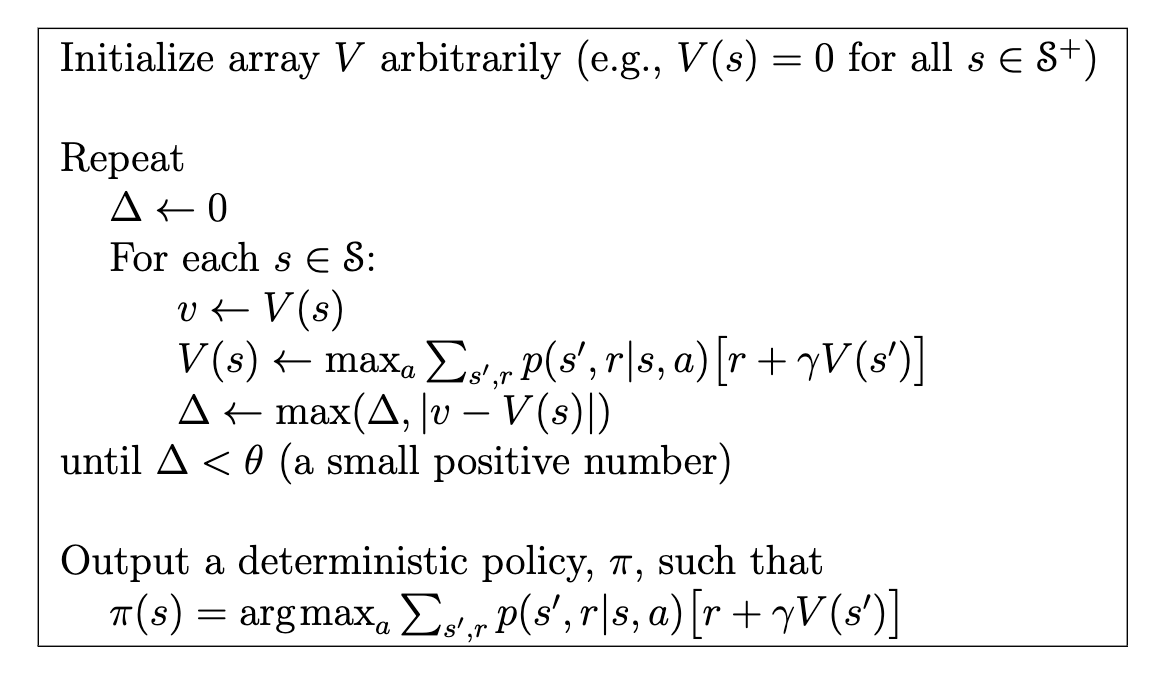
\includegraphics[scale=0.6]{p1.png}
\end{figure}

\paragraph{Contraction property of the Bellman operator}
\begin{align}
	||T^*Q_1 - T^*Q_2 ||_{\infty} &= ||Q_2 - Q_3 ||_{\infty}\\
	 &\leq \gamma||Q_1 - Q_2||_{\infty}
\end{align}
Equivalently,
$$\underset{(s,a)\in \mc{S} \times \mc{A}}{\sup} |(T^*Q_1)(s,a) - (T^*Q_2)(s,a)| \leq \underset{(s,a)\in \mc{S} \times \mc{A}}{\sup} |Q_1(s,a) - Q_2(s,a)|$$
\paragraph{Theorem}
By the Contraction property of the Bellman operator, the Value Iteration converges to the optimal value function.\\
\tb{Case 3: } If $\mc{S} \subset \real^d$ or $|\mc{S} \times \mc{A}|$ is very large:
Exact representation of the value function is infeasible for all $(s,a) \in \mc{S} \times \mc{A}$. The exact integration in the Bellman operator is challenging:
$$Q_{k+1}(s,a) \leftarrow r(s,a) + \gamma\int_{\textcolor{red}{\mc{S}}} \underset{a' \in \mc{A}}{\max}\, Q_k(s',a')\mc{P}(s'|s,a)\, ds'$$
We often do not know the dynamics $\mc{P}$ and the reward function $\mc{R}$, so we cannot calculate the Bellman operators.

\paragraph{Solution: Approximate/Fitted Value Iteration}
Suppose that we are given the following dataset
\begin{align}
	D_N &= \{(S_i, A_i, R_i, S'_i)\}_{i=1}^N \\
	(S_i, A_i) &\sim v \quad \text{$v$ is a distribution over $\mc{S} \times \mc{A}$} \\
	S'_i &\sim \mc{P}(\cdot|S_i, A_i) \\
	R_i &\sim \mc{R}(\cdot|S_i, A_i)
\end{align}
This is called \tb{Batch RL} problem. \\
We can approximately perform one step of Value Iteration using these data. \\
Consider a function $Q: \mc{S} \times \mc{A} \rightarrow \real$ \\
We can define a random variable $t_i = R_i + \gamma\,\underset{a' \in \mc{A}}{\max}\, Q(S'_i, a')$ \\
Notice that 
\begin{align}
	\mb{E}[t_i|S_i, A_i] &= \mb{E}\left[ R_i + \gamma \underset{a' \in \mc{A}}{\max} \, Q(S'_i, a')|S_i, A_i \right] \\
	&= r(S_i, A_i) + \gamma \int \underset{a' \in \mc{A}}{\max}\, Q(s', a')\mc{P}(s'|S_i,A_o)\, ds' \\
	&= (T^*Q)(S_i, A_i) \\
	&= Q_{k+1}(S_i, A_i)
\end{align}
So we can treat the problem of estimating $Q_{k+1}$ as a regression problem with noisy data. We minimize the squared error:
$$Q_{k+1} \leftarrow \underset{Q \in \mc{F}}{argmin} \, \frac{1}{N} \sum_{i=1}^N \left | \underbrace{Q(S_i, A_i)}_{\text{current Q}} - (\underbrace{R_i + \gamma \underset{a' \in \mc{A}}{\max} \, Q_k(S'_i, a))}_{\text{true Q}}\right |$$
We run this procedure $K$-times. \\

\subsection{Q-Learning}
\paragraph{Online RL}
The agent continually interacts with the environment, updates its knowledge of the world and its policy, with the goal of achieving as much rewards as possible.\\
\paragraph{Q-Learning with $\epsilon$-Greedy Policy}
Update the estimate of the action-value function $Q$ online and only based on $(S_t, A_t, R_t, S_{t+1})$, using the policy $\pi_t$ to explore the environment, such that $Q$ converges to the optimal value function $Q^*$.
\begin{itemize}
	\item learning rate $\alpha$, exploration parameter $\epsilon$
	\item Initialize $Q(s,a)$ for all $(s,a) \in \mc{S} \times \mc{A}$
\end{itemize}
The agent starts at state $S_0$. For time step $t= 0,1,\hdots$, choose $A_t$ according to the $\epsilon$-greedy policy
$$\pi_\epsilon(S_t; Q) = A_t \leftarrow \begin{cases}
	\underset{a \in \mc{A}}{argmax} \, Q(S_t,a) &\text{with probability $1-\epsilon$} \\
	\text{Uniformly random action in $\mc{A}$} &\text{with probability $\epsilon$}$$
\end{cases}$$
Take action $A_t$ in the environment. \\
The state of the agent changes from $S_t$ to $S_{t+1} \sim \mc{P}(\cdot|S_t, A_t)$. \\
Observe $S_{t+1}$ and $R_t$. \\
Update the action-value function at state-action $(S_t, A_t)$:
$$Q(S_t, A_t) \leftarrow\ Q(S_t, A_t) + \alpha\left[ R_t + \gamma \underset{a' \in \mc{A}}{\max} \, Q(S_{t+1}, a') - Q(S_t, A_t) \right ] $$

\paragraph{Remarks}
The $\epsilon$-greedy policy ensures that most of the time the agent exploits ints incomplete knowledge of the world by choose the best action, but occasionally it explores other actions. \\
One can show that under certain conditions, Q-Learning indeed converges to the optimal action-value function $Q^*$ for finite state-action spaces.

\subsection{Approaches to RL}
\begin{itemize}
	\item Discussed are \tb{value-based methods}: Optimize the value function
	\item \tb{policy search methods}: Optimize the policy
	\item \tb{Model-based RL}: Estimate the true, but unknown, model of environment $\mc{P}$ by an estimate $\hat{\mc{P}}$, and use $\hat{\mc{P}}$ to plan
	\item hybrid methods
\end{itemize}

    
\end{document}